% ######################################################################################################################
%         Foundations
% ######################################################################################################################

\chapter{Foundations}
\label{ch:Foundations}

\paperbox{
    This chapter is partially based on the peer-reviewed publications:
}{\paperart \paperpppp}{
    \todo{
        \textbf{Contributions:} Lucas Czech... Pierre Barbera... Alexandros Stamatakis... and...
    }
}

\todo{In this chapter, we introduce\ldots}

% ######################################################################################################################
%         Evolution and Genetics
% ######################################################################################################################

\section{Evolution and Genetics}
\label{ch:Foundations:sec:EvolutionGenetics}

% Evolution is change in the heritable characteristics of biological populations over successive generations.
% \url{https://en.wikipedia.org/wiki/Evolution}
% the process by which new species or populations of living things develop from preexisting forms through successive generations
% \url{https://www.merriam-webster.com/dictionary/evolution}
% Evolution is a process of continuous branching and diversification from common trunks. This pattern of irreversible separation gives life's history its basic directionality. —Stephen Jay Gould
% \url{https://www.merriam-webster.com/dictionary/evolution}

% Evolution is the continuous process of diversification of biological populations through successive generations \cite{Hall2008}.

Life on Earth is at least 3.77 billion years old \cite{Dodd2017},
and is continuously evolving due to \emph{natural selection} \cite{Darwin1859}.
% Woah, I like that very first sentences. A very old and a very new publication, binding all of reasearch together...
Driven by \emph{variation}, biological populations diversify through successive generations,
leading to the origination of new species.
This continuous process is called \emph{evolution} \cite{Hall2008}.
Heritable characteristics are passed down from parent to offspring,
with occasional random mutations leading to variation.
Thus, some organisms are better adapted to their environment than others,
and have more reproductive success.
There is hence a natural selection for advantageous mutations,
which can then spread through generations.

% this process was not understood for a long time. static species?
% four driving forces of pop gen?

The characteristics and traits of an organism are carried by, and inherited via, \emph{deoxyribonucleic acid} (DNA).
DNA is the molecule that encodes the genetic information needed for the functioning of all living organisms.
It is structured in form of a double helix \cite{Watson1953},
and built from two strands of molecules called \emph{nucleotides}.
The nucleotides build the backbone of the double helix,
and connect the two strands via opposing pairs of \emph{nucleobases}.
The redundant structure of pairs of nucleobases gives stability to the DNA molecule,
and also serves as a mechanism of error correction when reading the genetic information.
% both of which is important for the role of DNA for information storage.
In DNA, there are four distinct nucleobases:
adenine (\nucleobase{A}), cytosine (\nucleobase{C}), guanine (\nucleobase{G}), and thymine (\nucleobase{T}),
where \nucleobase{A} pairs with \nucleobase{T}, and \nucleobase{C} pairs with \nucleobase{G}, respectively.

\todo{explain transition vs transversion?}
\todo{picture of dna and the bases?}

The sequence of nucleobases along the strands of DNA is what encodes the genetic instructions
used by all known living organisms.
Parts of the DNA encode for proteins,
which perform a plethora of different functions within organisms.
Proteins consist of long chains of amino acid residues, and
are assembled in a process called protein (bio)synthesis.
This is described by the central dogma of molecular biology \cite{Crick1958,Crick1970}:
First, DNA is \emph{transcribed} into the intermediary ribonucleic acid (RNA),
which is then \emph{translated} into the actual protein.

In each step of this process, the alphabet used to encode information differs.
While DNA uses the four nucleobases as described above,
in RNA, the nucleobase uracil (\nucleobase{U}) is used instead of thymine (\nucleobase{T}).
Proteins on the other hand are (mostly) build from a set of \num{20} standard amino acids.
The set of rules used by the molecular machinery for translating nucleobases into amino acids
is called the \emph{genetic code}:
In a DNA sequence, three consecutive nucleobases are needed to encode one amino acid \cite{Shu2017}.

The entirety of the genetic material of an organism, that is, its complete DNA sequence, is called its \emph{genome}.
A \emph{gene} is a sequence which codes for a molecule that has a particular function, such as a protein \cite{Gericke2007}.
DNA and genes are the basic units of heredity.
They are what is varying across generations,
and what is selected for in the process of natural selection \cite{Dawkins1989}.
The study of genes, variation and heredity is called \emph{genetics} \cite{Griffiths2000}.

All life on this planet is related to each other and descends from a common ancestor.
Still, it is remarkable that the basic molecular principles and mechanisms of life---%
DNA, amino acids, and the genetic code---are virtually identical for all living organisms.
This implies that by understanding and comparing the genetic information encoded in the DNA of different organisms,
one can understand the diversification patterns of evolution.

% ######################################################################################################################
%         Sequence Analysis
% ######################################################################################################################

\section{Sequence Analysis}
\label{ch:Foundations:sec:SequenceAnalysis}

\todo{maybe move the paragraph above to here, and make a transition}

% ======================================================================================================================
%     Genome Sequencing
% ======================================================================================================================

\subsection{Genome Sequencing}
\label{ch:Foundations:sec:SequenceAnalysis:sub:GenomeSequencing}

Prior to analyzing the DNA of an organism, the physical order of nucleobases in the DNA molecule has to be determined.
That is, the DNA has to be ``read'' and stored in a human-accessible text format, typically a computer file.
This technical process is called DNA \emph{sequencing}.
% which can be understood as putting biomass into a blender and converting it into text files ;-)

For many decades, the main technique for this purpose was Sanger sequencing \cite{Sanger1975,Sanger1977}.
It is labor- and time-intensive, but through improvement and automation, costs were constantly reduced.
Eventually, this allowed for large-scale efforts, such as the Human Genome Project \cite{Venter2001},
which sequenced the whole human genome of more than three billion nucleobases.
Sanger sequencing allows to determine long parts of the sequence at once (> \num{500} nucleobases),
which then have to be assembled to build the final sequence.

In the last decades, a variety of novel high-throughput DNA sequencing technologies
have been developed \cite{Pettersson2009,Reuter2015,Deiner2017b}.
In particular, \emph{Next Generation Sequencing} (NGS) \cite{Logares2012,Mardis2013}
has revolutionized biology by transforming it into a data-driven and compute-intense discipline \citep{Escobar-Zepeda2015}.
The costs of these technologies are decreasing faster than Moore's law \cite{Wetterstrand2018}.
This leads to a ``tsunami'' of sequence data,
which poses a challenge for computational methods working with these data.
Compared to Sanger sequencing, NGS technologies are generally cheaper and faster \cite{Voelkerding2009,Metzker2010},
but come at the price of introducing more errors in the sequence output,
or only being able to determine shorter parts of the sequence at once
-- both of which constitute a challenge for the subsequent assembly of the final sequence.

The result of DNA sequencing is a textual representation of the order of nucleobases.
Although this representation ignores the physical and chemical properties of the respective molecules,
it is helpful in many applications, and allows to leverage existing algorithms.
Each contiguous sequence coming from the sequencing machine is called a \emph{read}.
Because of the pairing of nucleobases,
both DNA strands can be sequenced, which provides a means of error correction.
Such data are typically stored in the \fileformat{fastq} file format \citep{Cock2009}.
These so-called paired-end reads are then merged to form a final sequence representation of one strand
% cite \toolname{PEAR} \cite{Zhang2014} ?
-- that is, a sequence of the characters \nucleobase{A}, \nucleobase{C}, \nucleobase{G}, and \nucleobase{T}.
These data are stored in formats such as the \fileformat{fasta} file format \citep{Pearson1988}.
Due to the pairing of nucleobases,
the length of a DNA sequence is measured in \emph{base pairs} (abbreviated \si{\basepair}):
\SI{1}{\basepair} represents one character in the file.
These files are then the input for computational methods for working with DNA sequences.

% Not needed right now:
% Because of the universal genetic code of translating DNA to amino acids,
% it is also possible to store the amino acid sequence instead of the nucleobase sequence.

% ======================================================================================================================
%     Metagenomics
% ======================================================================================================================

\subsection{Metagenomics}
\label{ch:Foundations:sec:SequenceAnalysis:sub:Metagenomics}

Sanger sequencing requires careful preparation of the genetic material,
and is thus best used for sequencing single organisms.
There are however many (microbial) organisms that cannot be cultured in a Petri dish,
and are hence hard to sequence with this technique.
Apart from being cheaper, Next Generation Sequencing machines however ``digest'' all genetic material presented to them.
They thus allow for studying microbial samples
directly extracted from their environment \citep{Morgan2010,Edwards2013,Sunagawa2013a}.
This enables to study environments such as
water \cite{Karsenti2011,Giner2016,Gran-Stadniczenko2017},
soil \cite{Dupont2016,Mahe2017},
the human body \cite{Huttenhower2012,Methe2012,Srinivasan2012,Matsen2015},
and many others.
Each sample from such an environment then represents a geographical location, a body site, a point in time, etc.
% These studies yield a large set of short anonymous DNA reads for each sample.
% The DNA reads obtained from sequencing a sample represent all organisms present in the sample;
The DNA of all organisms being present in a sample is sequenced,
resulting in a large number of reads per sample.
These reads are anonymous, as it is unclear to which organism they originally belonged.

The study of these data, that is, genetic material from environmental samples, is called \emph{metagenomics} \cite{Oulas2015}.
% A first step is often to generate a genetic profile of the environment,
% that is, to estimate the diversity of the organisms in the sample.
A first step in such studies is often to characterize the reads obtained from an environment
in terms of \emph{reference sequences} of known species.
Reads that are similar to (parts of) reference sequences can be assigned to them,
while reads with low similarity to known sequences might indicate novel, undescribed species \cite{Temperton2012}.
Key tasks in metagenomic studies are the identification and classification of the anonymous reads (``Who is there?''),
and their functional annotation (``What are they doing?'') \cite{Desai2012}.
Both are introduced in the following.

% The following paragraph is not totally needed, as we are not doing functional analysis.
% However, it introduces many other terms alongside, which is useful later on.
Functional annotation \cite{Stein2001} is the prediction of gene functions of the reads,
and the inference of metabolic capacity of microbial communities \cite{Brown2017}.
As the proteins that are needed in the pathways of such functions can be encoded by genes across the genome,
whole-genome sequencing is necessary to capture all genes of interest.
For example, in shotgun sequencing \cite{Staden1979,Anderson1981},
the DNA is fragmented into small pieces within the size range that the used sequencing technology can handle,
typically a few hundred \si{\basepair} long.
This allows to sequence all genetic material contained in a sample.
Thus, the resulting reads originate from different parts of the genomes of their organisms,
which can then be functionally annotated \cite{Glass2010}.
This however necessitates to use whole-genome reference sequences
in order to be able to assign reads to known species and functions.
Typical databases of reference sequences however
lack many of the protein sequences from the microbial species present in a sample,
mostly because of organisms that cannot be cultured \cite{Brown2017}.

For the task of identification and classification of reads however, whole genome references are not needed.
Instead, specific \emph{marker genes} can be used,
which are regions of genes that are particularly suited for delineating between different species \cite{Ren2016}.
% highly conserved, that is, slowly changing over evolutionary times.
% but certain parts are radpidly evolung (hyper variable) withing the region, which is good for delineation.
% typically, this is general basic cell functionen stuff, which is needed by many forms of live.
% eg cell division, ssu... mitochondrial dna, etc
The method of using marker genes to identify species is called \emph{DNA barcoding} \cite{Hebert2003,Savolainen2005}.
The choice of genes to use as marker is important, and depends on the types of organisms to be studied.
The used marker genes should ideally be present in all of the organisms of interest,
short enough to be sequenced with current technology,
and have enough variation between species to distinguish between them,
but have low variation within species \cite{Kress2008}.

In many metagenomic studies of \taxonname{bacteria} and \taxonname{eukaryota},
the 16S \cite{Weisburg1991} and 18S \cite{Meyer2010} rRNA regions are used as marker genes,
respectively \cite{Woese1977,Woese1990}.
These regions belong to the small subunit (SSU) of the ribosomal ribonucleic acid (rRNA),
which is an essential component of the ribosome.
The ribosome is a molecular machinery that is responsible for protein synthesis (translation) in all living organisms.
% and are thus present in virtually all \taxonname{bacteria} and \taxonname{eukaryota}.
Often, prior to sequencing, these regions are amplified by many orders of magnitude,
using polymerase chain reaction (PCR) to create copies of these regions \cite{Bartlett2003}.
The resulting reads are then de-replicated again, which results in sequences called \emph{amplicons}.
While the PCR amplification process is known to introduce bias \cite{Logares2014,Brown2017},
this inexpensive method is commonly used in practice, particularly for the 16S and 18S rDNA regions.
A recent alternative to using PCR for obtaining reads from these regions are $_{\text{mi}}$tags \citep{Logares2014}.
In this approach, shotgun sequencing is used to get reads from the whole genomes of the organisms in a sample.
These reads are then filtered to only contain reads from the 16S region (for \taxonname{bacteria}),
which capture the diversity of the sample without bias.

Because of the ubiquity of the 16S and 18S rDNA regions in organisms and, consequently, in sequencing studies,
many databases provide reference sequences for these marker regions.
The reads or amplicons obtained from an environmental sample can then be employed
to estimate the microbial diversity of the organisms in the sample by comparison against known species.

% ======================================================================================================================
%     Sequence Alignments
% ======================================================================================================================

\subsection{Sequence Alignment}
\label{ch:Foundations:sec:SequenceAnalysis:sub:SequenceAlignment}

Organisms that evolved from a (not too distant) common ancestor share genetic information.
Regions of their DNA that have a shared ancestry are called \emph{homologous} regions \cite{Koonin2005}.
This homology is typically inferred from sequence similarity. %, that is, by comparison of the sequences.
However, due to mutations, differences in the sequences can occur.
There are three main types of sequence mutations that can occur in evolution:
a \emph{substitution} is the exchange of a nucleobase for another;
a \emph{insertion} adds one or more extra nucleotides into the sequence;
a \emph{deletion} removes one or more nucleotides from the sequence.
The latter two types of mutations change the length of the sequence;
a mutation that is either one of them is called an \emph{indel}.

Because of indels, sequences have to be aligned to each other in order to compare their homologous regions.
That is, gap characters (\nucleobase{-}) have to be added to the sequences
such that homologous characters in the sequence get aligned.
This results in an $n \times m$ matrix,
where $n$ is the number of sequences (rows),
and $m$ is the number of homologous characters (columns), called \emph{sites}.
This matrix is called a \emph{multiple sequence alignment} (MSA), or simply an \emph{alignment}.
\figref{fig:msa} shows an example of the alignment process and the resulting MSA.

\begin{figure}[hpbt]
    \centering
%     \vspace*{0.5em}
    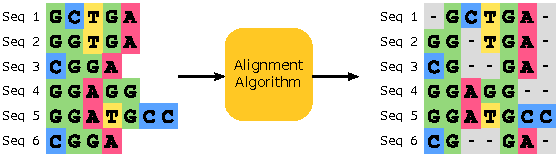
\includegraphics[width=.9\linewidth]{msa.pdf}
    \caption[Multiple Sequence Alignment]{
        \textbf{Multiple Sequence Alignment.}
        The left hand side shows a set of six sequences.
        Using an alignment algorithm, gaps are inserted into these sequences at presumed indel positions.
        The right hand side shows the result of this process,
        where homologous characters at the sites of the multiple sequence alignment (MSA) are aligned to each other.
        Below the MSA, the majority rule consensus sequence is shown,
        see \secref{ch:Foundations:sec:SequenceAnalysis:sub:ConsensusSequences}.
    }
    \label{fig:msa}
\end{figure}

Sequence alignment can be understood as an optimization problem under a given optimality criterion.
On the one hand, \emph{global alignments} attempt to align every character in every sequence,
which is most useful for similar sequences of roughly equal size.
For example, the Needleman-Wunsch algorithm \cite{Needleman1970} is a general global alignment technique
based on dynamic programming.
On the other hand, \emph{local alignments} are better suited for dissimilar sequences
which might contain similar regions within a larger sequence context.
The Smith-Waterman algorithm \cite{Smith1981} is a general local alignment technique
using the same dynamic programming scheme,
which additionally allows to start and end at any place in the sequence.
As both algorithms have their particular use cases \cite{Polyanovsky2011},
hybrid methods have also been developed \cite{Brudno2003}.
Furthermore, heuristic approaches such as \toolname{BLAST} \cite{Altschul1990} and
\toolname{USEARCH} \cite{Edgar2010} can calculate millions of near-optimal alignments in reasonable time.

These algorithms are efficient for the pairwise alignment of two sequences.
Calculating an MSA however has been shown to be NP-hard \cite{Wang1994,Just2001}.
Thus, for most empirical data sets, other approaches and heuristics are needed \cite{Thompson2011}.
Tools such as \toolname{CLUSTAL} \cite{Higgins1988}, \toolname{MUSCLE} \cite{Edgar2004}, and \toolname{MAFFT} \cite{Katoh2002}
can calculate near-optimal multiple sequence alignments for many thousands of sequences.

A special use case for aligning sequences arises in metagenomic studies,
where environmental sequences are often compared to a set of known reference sequences.
In these studies, one often first calculates an MSA of the reference sequences,
and then successively aligns the environmental sequences against this MSA.
This is because calculating an MSA for millions or billions of sequences from scratch is too expensive even for modern tools.
Hence, specialized algorithms for this use case have been developed,
such as \toolname{PaPaRa} \citep{Berger2011a,Berger2012} and
\toolname{hmmalign}, which is a subprogram of the \toolname{HMMER} suite \citep{Eddy1998,Eddy2009}.

% ======================================================================================================================
%     Consensus Sequences
% ======================================================================================================================

\subsection{Consensus Sequences}
\label{ch:Foundations:sec:SequenceAnalysis:sub:ConsensusSequences}

When working with a number of related but not identical sequences,
it is often convenient to ``summarize'' homologous characters in form of a \emph{consensus sequence}.
Such a sequence is typically calculated based on the relative frequencies of the characters per alignment site.
It then represents typical features and motifs of the input set of sequences.

The most straight forward method is to construct \emph{majority rule consensus} sequences \citep{May1952,Day1992a},
where each site is represented by the most frequent character at that site.
\figref{fig:msa} shows an example below the MSA on the right hand side.
In order to also include information from the less frequent characters at a site in the consensus sequence,
\emph{ambiguity characters} can be used \cite{IUPAC1970}.
They allow to denote multiple alternative nucleobases as a single character.
For example, if the nucleobases \nucleobase{A} and \nucleobase{G} are similarly frequent at a site,
this site is represented by the ambiguity character \nucleobase{R}.
See \tabref{tab:AmbiguityCharacters} for the full list of character representations.

Using ambiguity characters allows for more involved consensus methods.
For example, \emph{threshold consensus} sequences \citep{Day1992a,Day1992} include the most frequent characters
that are needed to achieve some given frequency threshold (between \num{50}\% and \num{100}\%) per site,
and represent these characters by their ambiguity character.
Furthermore, many methods based on fixed thresholds have been proposed,
such as Cavener's method \citep{Cavener1987,Cavener1991a};
see \cite{Day1992a} for a critical comparison.

It is theoretically also possible to directly use the relative frequencies of characters per site
in the mathematical frameworks of many downstream analysis methods.
This would allow to leverage all of the information contained in the input set of sequences.
However, to our knowledge, there is no convention or file format to store such information,
and consequently, no way of forwarding this information to the respective tools.

% ######################################################################################################################
%         Tree of Life
% ######################################################################################################################

\section{The Tree of Life}
\label{ch:Foundations:sec:TreeOfLife}

The shared evolutionary history of life gives rise to a branching pattern,
where new \emph{lineages} split from a common ancestor.
This branching pattern forms a tree-like structure,
which classifies organisms in a hierarchy based on common descent.

While this \emph{tree of life} is an expedient and, hence, pervasive model \cite{Mindell2013},
it ignores certain biological and evolutionary events.
A strict hierarchy does not allow for reticulate events,
such as hybridization \cite{Maddison1997a}, genetic recombination \cite{Hein1993},
or horizontal gene transfer \cite{Ochman2000,DunningHotopp2011,Robinson2013}.
Although approaches such as networks have been proposed to model these events \cite{Huson2011a},
the simplicity of a hierarchy or tree structure still has proven
to be useful in classifying and naming organisms, and understanding their evolutionary relationships.

% not considering lat gene tranfs, there is only one ``true'' tree of life.

% For the \taxonname{eukaryota}, the tree model is still considered valid.
% However, \taxonname{bacteria} have the ability of horizontal gene transfer,
% where genetic information is transferred between unrelated organisms.

% biology is messy: https://www.ncbi.nlm.nih.gov/pubmed/20852602

% ======================================================================================================================
%     Taxonomy and Nomenclature
% ======================================================================================================================

\subsection{Taxonomy and Nomenclature}
\label{ch:Foundations:sec:TreeOfLife:sub:TaxonomyNomenclature}

Early attempts at classifying organisms date back to the Greek philosopher Aristotle,
who used observable attributes to divide living things into groups \cite{Leroi2014}.
This approach as well as the efforts of later centuries were non-uniform and inconsistent.
The basis for the modern system of classification was established
by Swedish botanist Carl Linnaeus in the mid-18th century \cite{Donk1957}.
He proposed a \emph{nomenclature}, that is, a naming system for organisms,
as well as a \emph{taxonomy}, that is, a rank-based classification of organisms \cite{Linnaeus1735,Linnaeus1753}.

A taxonomic group of organisms is called a \emph{taxon} (plural: \emph{taxa}).
Each taxon is associated with a \emph{taxonomic rank}, which can subsume other ranks,
thus forming a hierarchy of higher and lower ranks.
A taxonomic rank represents the relative level of a group of organisms in the taxonomy.
The principal ranks in modern use are \taxonname{domain}, \taxonname{kingdom}, \taxonname{phylum}, \taxonname{class},
\taxonname{order}, \taxonname{family}, \taxonname{genus}, and \taxonname{species},
see \figref{fig:taxonomic_ranks}.
If needed, further ranks can be included in between (such as \emph{sub-genus}),
or more refined lower levels be added (such as \emph{strain}, which is a further distinction within a species).

\begin{figure}[hpbt]
    \centering
%     \vspace*{0.5em}
    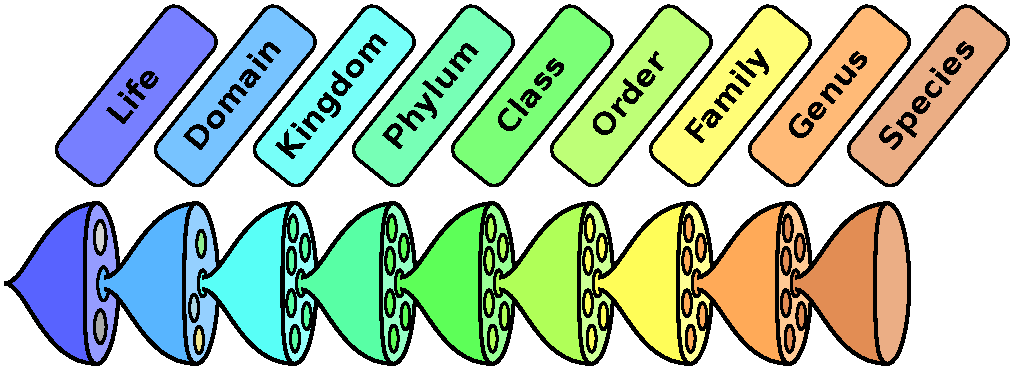
\includegraphics[width=.85\linewidth]{taxonomic_ranks.pdf}
    \caption[Biological classification into taxonomic ranks]{
        \textbf{Biological classification into taxonomic ranks.}
        The figure depicts a typical set of nested taxonomic ranks \cite{Woese1990},
        which form a hierarchy with increasingly deeper levels towards the right.
%         The taxonomic ranks shown here follow the three-domain system \cite{Woese1990}.
%         which classifies cellular life into the domains \taxonname{archaea}, \taxonname{eukaryota}, and \taxonname{bacteria}.
%         The deeper levels towards the right form a hierarchy of nested taxonomic ranks.
        Source: Image derived from \cite{Halasz2007}.
    }
    \label{fig:taxonomic_ranks}
\end{figure}

In order to scientifically name the groups of organisms (taxa) in a taxonomy,
the \emph{binomial nomenclature} as introduced by Linnaeus is still prevalent to this day.
It uses two terms, often of Latin origin,
which respectively specify the taxonomic ranks \emph{genus} and \emph{species} that an organism belongs to,
for example \taxonname{Homo sapiens}.

While early classifications used \emph{phenotypes}, that is, observable characteristics or traits of organisms,
modern approaches to taxonomy take genetic information into account \cite{Mayr2002}.
For example, the three-domain system \cite{Woese1977,Woese1990} resolves the oldest evolutionary relationships,
that is, the highest taxonomic levels, based on 16S rRNA data.
Although this classification has been challenged \cite{Gupta1998,Mayr1998,Cavalier-Smith2002}, it is widely used.
It divides cellular life forms into the three domains \taxonname{bacteria}, \taxonname{archaea}, and \taxonname{eukaryota};
the latter is further separated into kingdoms,
which include the kingdoms \taxonname{fungi}, \taxonname{plants}, and \taxonname{animals}.

% Archaea, Domain (and Kingdom)
% Eukarya, Domain
% Protista, Kingdom
% Fungi, Kingdom
% Animalia, Kingdom
% Plantae, Kingdom
% Bacteria, Domain (and Kingdom)

% ======================================================================================================================
%     Phylogenetic Trees
% ======================================================================================================================

\subsection{Phylogenetic Trees}
\label{ch:Foundations:sec:TreeOfLife:sub:PhylogeneticTrees}

The classification of organisms into a taxonomy is based on (subjective) dissimilarity and thus arbitrary:
The number of organisms that are grouped into a taxon at a given rank can vary,
and the separation into discrete ranks does not reflect the gradual nature of evolution \cite{Gingerich1987}.
A more involved approach that can resolve these issues is \emph{phylogenetics},
which is the study of the evolutionary history and relationships of biological entities (individuals, species, populations).

The evolutionary relationships of such entities are called their \emph{phylogeny}.
As the true phylogeny of a set of taxa is unknowable,
it has to be inferred from data that is available.
A phylogenetic analysis uses inference methods that evaluate observed heritable traits
in order to resolve the phylogeny under a given model of evolution of these traits.
While phenotypes can be used, modern phylogenetic inference is mostly based on DNA data.
The result of a phylogenetic analysis is a \emph{phylogenetic tree},
also called an \emph{evolutionary tree}, or---synonymously---a \emph{phylogeny}.
\figref{fig:tree_of_life} shows two examples of phylogenetic trees.

\begin{figure}[hpbt]
    \centering
    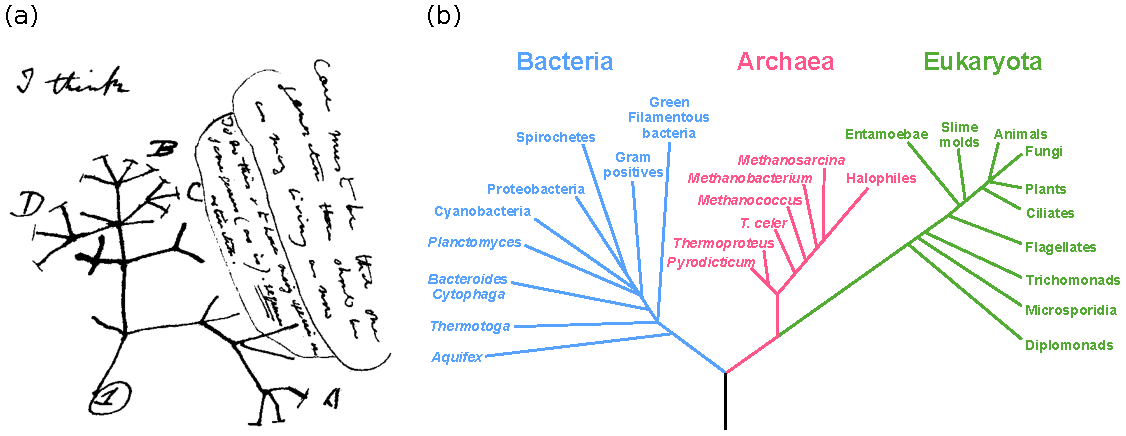
\includegraphics[width=\linewidth]{tree_of_life.pdf}
    \begin{subfigure}{0pt}
        \phantomcaption
        \label{fig:tree_of_life:sub:darwin}
    \end{subfigure}
    \begin{subfigure}{0pt}
        \phantomcaption
        \label{fig:tree_of_life:sub:woese}
    \end{subfigure}
    \caption[Exemplary phylogenetic trees]{
        \textbf{Exemplary phylogenetic trees.}
        \subref{fig:tree_of_life:sub:darwin}
        In 1837, Charles Darwin sketched his first evolutionary tree below the words ``I think''
        in his notebook on ``Transmutation of Species''.
        Source: Image derived from \cite{DarwinTreeOfLife1837}.
%         \\
        \subref{fig:tree_of_life:sub:woese}
        A modern phylogenetic tree showing the three-domain system \cite{Woese1977,Woese1990},
        which emphasizes the separation of \taxonname{bacteria}, \taxonname{archaea}, and \taxonname{eukaryota}
        based on 16S rRNA genes.
        The black branch at the bottom represents the speculative last universal common ancestor of all living organisms.
        Source: Image derived from \cite{WoeseTreeOfLife2006}.
    }
    \label{fig:tree_of_life}
\end{figure}

The leaf nodes, or \emph{tips}, of the tree represent living (\emph{extant}) biological entities
such as species, strains, individual organisms, or even cells of a multicellular organism.
Thus, the tips are often referred to as the \emph{taxa} of the tree,
which is meant as a generic term that includes all the above entities.
The tips are often named according to the entities they represent (e.\,g., species names);
such a tree is called a \emph{labeled} tree.
The inner nodes on the other hand are usually anonymous and
represent speciation events, where two novel lineages arose from a putative common ancestor.
The branching pattern of a phylogenetic tree thus reveals the evolutionary history of its taxa.

The edges of the tree, also called its \emph{branches}, can have associated \emph{branch lengths},
which represent the evolutionary time between the two adjacent nodes,
for example, measured as the average change in nucleobases between their respective sequences.
The unique path between any two nodes thus can be interpreted
as a measure of evolutionary relatedness of the taxa represented by the nodes.

A phylogenetic tree is \emph{rooted}
if it is a directed tree that has a unique \emph{root node},
which corresponds to the putative common ancestor of the other nodes in the tree.
See \figref{fig:tree_of_life:sub:woese} for an example.
As evolution is a processes that happens over time,
from a biological point of view, every tree has a root.
However, most models of DNA evolution are time-reversible,
meaning that the direction of change in the sequences cannot be inferred from the data,
see \secref{ch:Foundations:sec:TreeOfLife:sub:TreeInference:par:ModelsOfSeqEvol} for details.
Thus, tree inference methods can also yield \emph{unrooted} trees without direction and without a root node.
These can be rooted a posteriori, for example by using an \emph{outgroup} of taxa
that are closely related to the group of taxa of interest (the \emph{ingroup}), but not part of it.
Then, a root node can be placed on the branch that separates the outgroup from the ingroup.

An inner node that has exactly three neighboring nodes is called a \emph{bifurcation} or a \emph{bifurcating} node.
In rooted trees, these neighbors are the the parent and the two children of a node, hence the name.
An inner node with more neighbors is called a \emph{multifurcation} or a \emph{multifurcating} node.
This naming also applies to the whole tree:
A tree, where each inner node (with the exception of the root node in a rooted tree) is bifurcating,
is also called a bifurcating tree.
Otherwise (if there is at least one multifurcating node), it is a multifurcating tree.
Note that in evolution, an actual multifurcation event is highly unlikely,
as it corresponds to the simultaneous formation of more than two new lineages from a single ancestral lineage.
Multifurcating trees are for example used when relationships cannot be properly resolved from the existing data,
or to summarize a set of otherwise contradicting trees.

Each edge of the tree induces a \emph{bipartition} or \emph{split} of the taxa of the tree into two groups,
one on each side of the edge.
A set of taxa is \emph{monophyletic},
if there is a bipartition of the tree that splits these taxa from all other taxa of the tree.
In a rooted tree, the node at the end of that edge is then the putative common ancestor of these taxa.
Furthermore, a monophyletic set of taxa is called a \emph{clade} of the tree;
in other words, a clade is a subtree that is separated from the rest of the tree by one edge.
For example, the taxa {\sffamily A}, {\sffamily B}, and {\sffamily C} in \figref{fig:tree_vis_options} are monophyletic---%
that is, they form a clade of the tree.
Lastly, a non-monophyletic set of taxa is \emph{paraphyletic}.

While the topology of the tree is what models the evolutionary relationships,
there are several ways of visualizing or drawing that information.
\figref{fig:tree_vis_options} shows some examples, which all visualize the same topology (except for the rooting).
The figure also summarizes some of the terms and concepts introduced above.
Different drawing styles each have their advantages.
For example, in a rectangular tree (\figref{fig:tree_vis_options:sub:rectangular}),
branch lengths are easier to read and compare,
while a circular tree (\figref{fig:tree_vis_options:sub:circular}) can fit more taxa in the same drawing area.

\begin{figure}[hpbt]
    \centering
    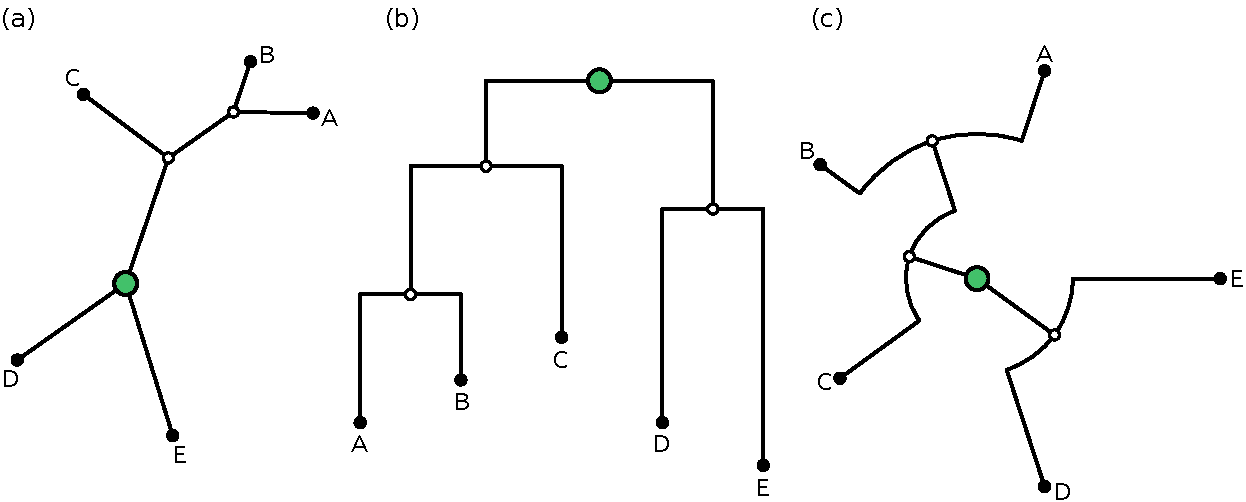
\includegraphics[width=\linewidth]{tree_vis_options.pdf}
    \begin{subfigure}{0pt}
        \phantomcaption
        \label{fig:tree_vis_options:sub:unrooted}
    \end{subfigure}
    \begin{subfigure}{0pt}
        \phantomcaption
        \label{fig:tree_vis_options:sub:rectangular}
    \end{subfigure}
    \begin{subfigure}{0pt}
        \phantomcaption
        \label{fig:tree_vis_options:sub:circular}
    \end{subfigure}
    \caption[Types of phylogenetic trees]{
        \textbf{Types of phylogenetic trees.}
        Here, we show three different types of labeled, bifurcating trees.
        Tip nodes are marked with black dots, inner nodes with white dots, and the root node (if present) with a green dot.
        \subref{fig:tree_vis_options:sub:unrooted} An unrooted tree with five taxa.
        \subref{fig:tree_vis_options:sub:rectangular} The same tree topology,
        but rooted on the inner branch that splits the taxa {\sffamily D} and {\sffamily E} from the other taxa.
        The tree is drawn in rectangular style.
        \subref{fig:tree_vis_options:sub:circular} The same tree again, but this time drawn in circular style.
    }
    \label{fig:tree_vis_options}
\end{figure}

Taxonomy and phylogeny serve a related, but different purpose:
While the former is a system of classification,
the latter reveals evolutionary history.
However, there is a correspondence between a taxonomy and a rooted phylogeny:
Inner nodes of the tree constitute older evolutionary relationships,
which are represented by the higher ranks of the taxonomy.
\figref{fig:tree_of_life:sub:woese} shows such a correspondence for the three domains of life.
It is however possible that the taxa at one rank of the taxonomy are not monophyletic in the tree.
In this case, the two are \emph{incongruent}.

% particularly considering that the genes might evolve differently from the species or from what the taxonomy says

The most common file format for storing phylogenetic trees is the \fileformat{Newick} format \cite{Archie1986},
which uses parentheses and commas to specify the nesting structure of the tree,
and allows to store node labels and branch lengths.
The \fileformat{NEXUS} format \cite{Maddison1997} is a container format for biological data,
and internally also relies on the \fileformat{Newick} format for storing trees.
Furthermore, the \fileformat{phyloXML} format \cite{Han2009} is an \fileformat{XML} based format
that allows to store arbitrary data at the nodes and edges of the tree.
% This is particularly useful for annotating the tree with additional data.

% ======================================================================================================================
%         Tree Inference
% ======================================================================================================================

\subsection{Tree Inference}
\label{ch:Foundations:sec:TreeOfLife:sub:TreeInference}

A phylogeny can be inferred from data that has per-taxon traits which are homologous,
that is, which have evolved from the same traits in the common ancestor and are thus comparable \cite{Felsenstein2004,Yang2006}.
While historically these traits were mostly phenotypes (bone shapes and sizes, metabolism, etc.),
the focus has since shifted towards molecular data such as DNA and amino acid sequences,
as their \emph{phylogenetic signal} is generally more abundant and less biased \cite{Hillis2000}.
Most often, a multiple sequence alignment is used,
whose homologous sites represent the traits of the taxa.
To determine the degree of relatedness between taxa, mathematical models of trait evolution are employed.

% Searching the tree space
The general concept of tree inference is then to put closely related taxa close to each other in the phylogeny.
Hence, a tree inference can be thought of as an optimization problem,
which searches for the best tree given an optimality criterion.
However, the space of all possible tree topologies is too large for an exhaustive brute-force search
for virtually all empirical datasets.
For a given number of taxa $n$, the number of distinct tree topologies N is given as
$N(n) = \prod_{\,i=3}^{\,n} ~(2i - 5)$,
which grows over-exponentially fast \cite{Felsenstein2004}.
There are thus different approaches and heuristics to conduct tree search.

% Methods overview
Distance based methods such as \emph{Unweighted Pair Group Method with Arithmetic Mean} (UPGMA) \cite{Sokal1958}
and \emph{Neighbor Joining} \cite{Saitou1987}
use a pairwise distance matrix between sequences, and thus do not necessarily need an alignment.
\emph{Maximum Parsimony} \cite{Sankoff1975} uses an optimality criterion that is based on Occam's razor,
that is, it yields the tree that explains the observed tip sequences (taxa)
with the minimal number of substitutions (mutations).
The \emph{Maximum Likelihood} (ML) method \cite{Felsenstein1981} employs statistical techniques
in order to evaluate the probability of a given phylogenetic tree with respect to a given alignment,
and successively search the tree space for the most likely tree.
Furthermore, \emph{Bayesian Inference} also relies on the evaluation of tree probability \cite{Yang2006},
and uses Bayes' theorem to calculate the posterior distribution of the relevant evolutionary processes;
it thus can incorporate prior empirical knowledge into the process.

\paragraph{Maximum Likelihood Tree Inference}
\label{ch:Foundations:sec:TreeOfLife:sub:TreeInference:par:MLTreeInference}

% Maximum Likelihood
In the context of this work, we are mostly interested in Maximum Likelihood (ML) tree inference.
It uses a probabilistic framework in which the (phylogenetic) likelihood

\begin{equation}
    L(~ \mbox{MSA} ~|~ T, \bar{b}, M, \bar{\theta} ~)
\end{equation}

is evaluated that an observed MSA is the outcome of an evolutionary history described by a phylogenetic tree
with topology $T$ and branch lengths $\bar{b}$, under a given model of trait evolution $M$ with parameters $\bar{\theta}$.
For a fixed model $M$ (see below), the likelihood can be expressed as a function of $T$, $\bar{b}$ and $\bar{\theta}$,
which is known as the \emph{phylogenetic likelihood function} (PLF).
By maximizing the PLF using maximum likelihood estimation,
the parameter values (including tree topology) are found which best explain the observed data.
These estimates are typically obtained by iteratively and independently optimizing
the tree topology and the branch lengths and model parameters,
which is introduced in the following.

% Optimizing the topology:
Finding the most likely tree topology is a discrete optimization problem,
which has been shown to be NP-hard under the ML criterion \cite{Chor2005}.
Furthermore, the evaluation of the PLF is computationally expensive,
as it involves many floating point operations.
A general heuristic for the tree search that avoids an exhaustive evaluation of the tree space is thus as follows.
First, a starting tree is generated, either randomly, or using methods such as Neighbor Joining or Maximum Parsimony.
Then, the likelihood of the tree is successively improved
by applying topological rearrangements (\emph{moves}) of its taxa and clades.
For instance, in \emph{greedy hill-climbing} \cite{Stamatakis2014}, only those moves are applied (\emph{accepted})
that immediately improve the PLF, until a (potentially local) optimum is found.

%Optimizing branch lengths and model parameters:
For a fixed tree topology $T$, the maximum likelihood estimates
of the branch lengths $\bar{b}$ and the model parameters $\bar{\theta}$
are usually obtained with general-purpose numerical optimization methods.
Since the derivatives of the PLF can be easily computed,
the Newton-Raphson method \cite{Ypma1995} is often used for optimizing the branch lengths.
Model parameters are commonly optimized with Brent's method \cite{Brent1971}
or with the Broyden-Fletcher-Goldfarb-Shanno (BFGS) algorithm \cite{Fletcher1987}.

\paragraph{Models of Molecular Sequence Evolution}
\label{ch:Foundations:sec:TreeOfLife:sub:TreeInference:par:ModelsOfSeqEvol}

% Models of molecular sequence evolution
So far, we assumed a fixed model $M$ for describing the evolution of the traits that are used for inferring the tree.
For sequence data, such a model yields an estimate of the evolutionary distance between the sequences of different taxa.
Most commonly, a continuous-time Markov chain (MC) is used to describe
the evolution of a single site within a set of aligned sequences \cite{Gagniuc2017}.
For DNA data, the MC has four states \nucleobase{A}, \nucleobase{C}, \nucleobase{G}, and \nucleobase{T},
which correspond to the nucleobases, and transitions between the states correspond to their substitutions,
see \figref{fig:mc_state_transitions}.
While the MC model ignores aspects such as natural selection and the molecular mechanisms of evolution,
it describes the relative rate of changes in a way that allows multiple substitutions to occur
along the same branch (\nucleobase{T} $\rightarrow$ \nucleobase{A} $\rightarrow$ \nucleobase{G}).
\todo{if transition vs transversion is explained above, we need to clarify here:
note that transition is used in two different meanings here...}

\begin{figure}[hpbt]
    \centering
    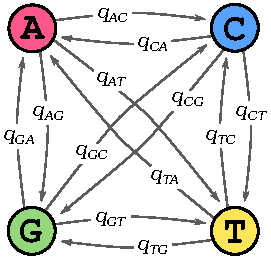
\includegraphics[width=.35\linewidth]{mc_state_transitions.pdf}
    \caption[Markov chain model of nucleotide substitutions]{
        \textbf{Markov chain Model of Nucleotide Substitutions.}
        The evolution of characters at a site in an alignment can be modeled as a Markov chain (MC).
        The states of the MC for DNA data are the four nucleobases
        \nucleobase{A}, \nucleobase{C}, \nucleobase{G}, and \nucleobase{T}.
        The model allows transitions with rates $q_{ij}$ with $i,j \in \left\{~ A, C, G, T ~\right\}, i \neq j$ between all states,
        which correspond to substitutions of the nucleobases.
    }
    \label{fig:mc_state_transitions}
\end{figure}

% \begin{figure}[hpbt]
%  \begin{subfigure}[c]{.5\textwidth}
%     \centering
%     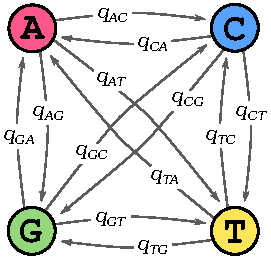
\includegraphics[width=.7\linewidth]{mc_state_transitions.pdf}
%     \caption{}
%     \label{fig:mc_state_transitions:sub:mc_chain}
%  \end{subfigure}
%  \begin{subfigure}[c]{.5\textwidth}
%     \begin{align*}
%         Q ~&=~
%          \begin{pmatrix}
%          ~-q_{A}   &   q_{AC}   &   q_{AG}   &   q_{AT}~~ \\
%          ~q_{CA}   &  -q_{C}    &   q_{CG}   &   q_{CT}~~ \\
%          ~q_{GA}   &   q_{GC}   &  -q_{G}    &   q_{GT}~~ \\
%          ~q_{TA}   &   q_{TC}   &   q_{TG}   &  -q_{T}~~
%          \end{pmatrix}
%         \\ \\
%         - q_{i} ~&=~ - \sum_{j \neq i} q_{ij}, ~ i = \left\{~ A, C, G, T ~\right\}
%     \end{align*}
%     \caption{}
%     \label{fig:mc_state_transitions:sub:matrix}
%   \end{subfigure}
%     \caption[Markov chain model of nucleotide substitutions]{
%         \textbf{Markov chain Model of Nucleotide Substitutions.}
%         The evolution of characters at a site in an alignment can be modeled as a Markov chain (MC).
%         \subref{fig:mc_state_transitions:sub:mc_chain} The states of the MC for DNA data are
%         the four nucleobases \nucleobase{A}, \nucleobase{C}, \nucleobase{G}, and \nucleobase{T}.
%         The model allows transitions between all states, which correspond to substitutions between the nucleobases.
%         \subref{fig:mc_state_transitions:sub:matrix} The instantaneous transition rates between states are given
%         by the substitution rate matrix (Q-matrix), where the rows must sum to $0$.
%     }
%     \label{fig:mc_state_transitions}
% \end{figure}

The process of state transitions is defined by the substitution rate matrix %$Q$

\begin{equation}
    \begin{align*}
        Q ~&=~
         \begin{pmatrix}
         ~-q_{A}   &   q_{AC}   &   q_{AG}   &   q_{AT}~~ \\
         ~q_{CA}   &  -q_{C}    &   q_{CG}   &   q_{CT}~~ \\
         ~q_{GA}   &   q_{GC}   &  -q_{G}    &   q_{GT}~~ \\
         ~q_{TA}   &   q_{TC}   &   q_{TG}   &  -q_{T}~~
         \end{pmatrix}
        \\ \\
        - q_{i} ~&=~ - \sum_{j \neq i} q_{ij}, ~ i = \left\{~ A, C, G, T ~\right\}
    \end{align*}
\end{equation}

% The instantaneous transition rates between states are given
% by the substitution rate matrix (Q-matrix), where the rows must sum to $0$.
where the elements $q_{ij}$ are the \emph{instantaneous transition rates} from state $i$ to state $j$.
The rows of the matrix have the requirement to sum to $0$,
by which the diagonal elements $q_{i}$ are defined.

The branch lengths of a phylogeny express the evolutionary time between two nodes,
which can be interpreted as the expected number of substitutions between the respective alignment sites.
Then, for a given time $t$, the \emph{transition probabilities} $p_{ij}(t)$ between states in a stationary process
are obtained by exponentiating the $Q$ matrix \cite{Yang2006}.
These probabilities are specified by the matrix

\begin{equation}
    P(t) = e^{Qt}
\end{equation}

For positive transition rates $q_{ij} > 0, \forall i \neq j$, if the process runs long enough,
the Markov chain eventually reaches the unique \emph{stationary} distribution $\Pi = (\pi_A$, $\pi_C$, $\pi_G$, $\pi_T )$,
with $\pi_i$ being the proportion of time spent in state $i$.
If the Markov process reached equilibrium after running long enough,
it can be interpreted as generating the sequences of the MSA.
In that case, $\Pi$ is the \emph{equilibrium base composition} of the MSA,
and $\pi_i$ are the \emph{equilibrium} or \emph{stationary base frequencies} of the MSA.

As mentioned before, most models of DNA evolution assume a \emph{time-reversible} Markov process,
which means that $\pi_{i} q_{ij} = \pi_{j} q_{ji} ~ \forall \, i \neq j$.
This assumption is biologically not meaningful, as evolution is a process in time, and thus does have a direction.
It however allows for simplified calculations:
The $Q$ matrix of a time-reversible model can be formulated as the product of
a \emph{symmetric} rate matrix $R = \left\{ r_{i \leftrightarrow j} \right\}$ and
a diagonal matrix with the stationary base frequencies:

\begin{align}
    \newcommand{\lra}{\leftrightarrow}
    Q = R \cdot diag(\pi_i) =
    \begin{pmatrix}
         -q_A                       &   r_{A \lra C} \cdot \pi_C   &   r_{A \lra G} \cdot \pi_G   &   r_{A \lra T} \cdot \pi_T~~  \\
        ~r_{A \lra C} \cdot \pi_A   &   -q_C                       &   r_{C \lra G} \cdot \pi_G   &   r_{C \lra T} \cdot \pi_T~~  \\
        ~r_{A \lra G} \cdot \pi_A   &   r_{C \lra G} \cdot \pi_C   &   -q_G                       &   r_{G \lra T} \cdot \pi_T~~  \\
        ~r_{A \lra T} \cdot \pi_A   &   r_{C \lra T} \cdot \pi_C   &   r_{G \lra T} \cdot \pi_G   &   -q_T
    \end{pmatrix}
\end{align}

The matrix describes the most general model of DNA evolution,
where all \num{6} substitution rates $r_{i \leftrightarrow j}, i \neq j$ and
all \num{4} base frequencies $\pi_i$ can be different.
This model is called the Generalized Time-Reversible (\toolname{GTR}) model \cite{Tavare1986}.
As the sum of the base frequencies must be $1$,
and as the substitution rates are usually normalized by requiring that $r_{G \leftrightarrow T} = 1.0$,
the \toolname{GTR} model has a total of \num{8} free parameters
(that is, \num{3} base frequencies, and \num{5} substitution rates).

There are also more restrictive models, which have fewer free parameters,
and are thus more robust if data for estimating them is sparse.
The Jukes-Cantor model (\toolname{JC69}) \cite{Jukes1969} has no free parameter and assumes
equal substitution rates $r_{i \leftrightarrow j} = 1$, $i \neq j$ and equal base frequencies $\pi_i = \sfrac{1}{4}$.
The \toolname{K80} model \cite{Kimura1980} adds a free parameter $\kappa$,
which describes the ratio between two types of substitutions that are not equally likely to occur in evolution:
$r_{A \leftrightarrow C} = r_{G \leftrightarrow T} = \kappa \cdot r_{A \leftrightarrow G} =
\kappa \cdot r_{A \leftrightarrow T} = \kappa \cdot r_{C \leftrightarrow G} = \kappa \cdot r_{C \leftrightarrow T}$.
\todo{if transition vs transversion was added earlier, add it here, too!}einhalten
The \toolname{HKY85} model \cite{Hasegawa1985} further adds parameters for the base frequencies,
and hence has \num{4} free parameters.
Further models have also been proposed, which offer compromises
between the number of free parameters and the expressiveness of the model \cite{Yang2006}.

The state space of the Markov process becomes significantly larger for protein data,
as it needs to comprise \num{20} standard amino acids instead of \num{4} nucleobases.
Hence, the \toolname{GTR} model for protein data has $(400 - 20) / 2 - 1 + 19 = 208$ free parameters.
Typical amino acid alignments do not contain enough data to reliably estimate these parameters,
and thus easily lead to over-fitting.
Thus, so-called \emph{empirical} amino acid models are commonly used,
which have substitution rates and equilibrium base frequencies
that were pre-estimated on large collections of reference alignments.
Among others, some popular models include \toolname{DAYHOFF} \cite{Dayhoff1978},
\toolname{WAG} \cite{Whelan2001}, and \toolname{LG} \cite{Le2008}.

\paragraph{Further Aspects of Tree Inference}
\label{ch:Foundations:sec:TreeOfLife:sub:TreeInference:par:FurtherAspects}

Evolution is an incredibly complex process with intricate details.
Many more models and methods have thus been proposed to refine tree inference \cite{Yang2006},
of which we here briefly introduce a few.
% For understanding the methods described in this work, the above introduction should suffice.
% For the distinguished reader, we here still mention a few other aspects that are related to the topic.
% While a detailed description of these models and methods is not necessary for understanding the main chapters of this work,
% we here still mention a few other related aspects.

The models of sequence evolution described above make the simplifying assumption
that the alignment sites evolve independently and are identically distributed.
However, certain regions of DNA or amino acid sequences are under higher evolutionary pressure then others,
for example if they describe important molecular functions.
It is thus expected that some alignment sites evolve faster than others.
In the context of phylogenetic inference,
several models of \emph{rate heterogeneity among sites} have been proposed to account for this,
some of which are described in the following.
\\
A simple model is the \emph{proportion of invariable sites},
where the likelihood of an alignment site is influenced by a parameter $p \in [0,1]$
that describes the proportion of sites that are assumed to be identical (\emph{invariable}) across all taxa.
The more elaborate $\Gamma$ model \cite{Yang1994a} postulates a shape parameter $\alpha$
which models the rate heterogeneity as a gamma function $\Gamma(\alpha)$.
The distribution shape ranges from exponential-like ($\alpha < 1$, high rate heterogeneity)
to normal-like ($\alpha > 10$, low rate heterogeneity).
Thus, by optimizing the single free parameter $\alpha$, different rate heterogeneity profiles can be approximated.
Lastly, the \toolname{CAT} or \emph{per-site rates} model \cite{Stamatakis2006a}
is a compute- and memory-efficient approximation of the $\Gamma$ model,
which explicitly assigns one of $K$ rate categories to each alignment site instead of using a distribution of rates.

The tree search as described before can (theoretically) yield any topology from the vast space of possible trees.
It is however often serviceable to run a \emph{constrained} tree search,
for example to include prior knowledge about the taxa,
to maintain congruence with a given taxonomy, or because some other constraints are required.
Such a constraint can for example be specified by enforcing certain bipartitions to be retained in the tree,
that is, splits of the taxa that must be separated from each other in the tree.
As a bipartition is induced by a branch in the tree,
this is equivalent to starting the tree search with a multifurcating tree,
and then resolving these multifurcations without changing the other parts of the tree.
A constrained search yields a \emph{constrained tree}.

\todo{
Alignment Partitioning
Computation of Phylogenetic Likelihood Func-
tion and its Derivatives
    P-matrix
    Conditional Likelihood Vectors
    Likelihood Evaluation at the Root
    6.4
Likelihood Derivatives with respect to the Branch Length Parameter
}

% ######################################################################################################################
%         Phylogenetic Placement
% ######################################################################################################################

\section{Phylogenetic Placement}
\label{ch:Foundations:sec:PhylogeneticPlacement}

introduce ``reference tree'', as a tree inferred from reference sequences.

. common use case: fixed tree, selected by experts to consist of know, described taxa
to represent the diversity expected from an environment.


Since the amount of sequence data produced in metagenomic studies can be quite substantial,
computational challenges and bottlenecks arise \cite{Scholz2012}.


mention that epa ng can use all the model stuff explaine above: subst models, rate hetero, etc
allows gtr and always uses gamma

% ======================================================================================================================
%     Motivation
% ======================================================================================================================

\subsection{Motivation}
\label{ch:Foundations:sec:PhylogeneticPlacement:sub:Motivation}


problem with ngs data:
msa is NP-hard \cite{Just2001}.
inferring tree for this many sequences is also NP-hard \cite{Chor2005} even harder (over exp.), plus
short sequences (not phylo signal), so cannot resolve relationtips between sequences


% although the methods generally are applicable to both.
A typical task in metagenomic studies is to identify and classify these sequences with respect
to known reference sequences, either in a taxonomic or phylogenetic context.
% another typical task: to discover novel diversity. not here.

Conventional methods like \toolname{Blast} \cite{Altschul1990} are based on sequence similarity.
Such methods are fast, but only attain satisfying accuracy levels
if the query sequences (e.g., the environmental reads or amplicons) are sufficiently similar to the reference sequences.
Furthermore, the best \toolname{Blast} hit does often \emph{not} represent the most closely related species \cite{Koski2001}.
% \todo{Mention further methods here, for example Vervier 2015}
This is particularly true for environments where available reference databases
do not exhibit sufficient taxon coverage \citep{Mahe2017}.
As insufficient taxon coverage cannot be detected by methods that are based on sequence similarity,
they can potentially bias downstream analyses.

Alternatively, so-called phylogenetic (or evolutionary) placement methods \cite{Matsen2010,Berger2011,Barbera2018}
identify query sequences based on a phylogenetic tree of reference sequences.
Thereby, they incorporate information about the evolutionary history of the species under study
and hence provide a more accurate means for read identification.
The result of phylogenetic placement is a mapping of the query sequences to the branches of the reference tree.
Such a mapping also elucidates the evolutionary distance between the query and the reference sequences.

This information represents useful biological knowledge \emph{per se}.
For example, the classification of query sequences can be summarized by means of sequence abundances \cite{Pace1997,Hugenholtz1998},
or to obtain taxonomic annotations \cite{Kozlov2016}.
The data can also be utilized to derive further knowledge or hypotheses.
Existing methods such as Edge PCA and Squash Clustering \cite{Matsen2011a} are, for instance, able
to visualize differences between sets of metagenomic samples,
or to cluster samples based on placement similarity.
Note that distinct samples from one study are typically mapped to the same underlying reference tree,
thus facilitating such comparisons.



phylogenetic placement \cite{Matsen2010,Berger2011,Barbera2018}, cited more than 630 times (as of 2018-07-01)
considered an established method

There also exist variants of phylogenetic placement that use maximum parsimony \cite{Berger2011}
and minimum evolution \cite{Filipski2015} instead of maximum likelihood,
variants that calculate Bayesian posterior probabilities \cite{Matsen2010},
and boosting methods to improve the accuracy of the placements \cite{Mirarab2012}.
Phylogenetic placement has been used for a variety of applications and derived pipelines, such as
species delimitation \cite{Zhang2013,Kapli2017},
genome and metagenome analysis \cite{Darling2014},
taxonomic identification and phylogenetic profiling \cite{Nguyen2014}, and
identification and correction of taxonomically mislabeled sequences \cite{Kozlov2016}.

combine 1,010 more citations (as of 2018-07-01)
see also recent art version

there is also a recent approach that yields comparable results (also jplace), but uses an alignment-free, non ML approach \cite{Linard2018}.


aligning

kommt unten noch mal!

, using programs such as \toolname{PaPaRa} \citep{Berger2011a,Berger2012} or
\toolname{hmmalign}, which is a subprogram of the \toolname{HMMER} suite \citep{Eddy1998,Eddy2009}.

% ======================================================================================================================
%     Introduction
% ======================================================================================================================

\subsection{Introduction}
\label{ch:Foundations:sec:PhylogeneticPlacement:sub:Introduction}

\todo{pipeline diagram, data flow, etc, reference to chapters?!}

In brief, phylogenetic placement calculates the most probable insertion branches for each given \acf{QS} on a \acf{RT}.
The \acp{QS} are reads or amplicons from environmental samples; most often barcoding regions or marker genes are used.
The \ac{RT} and the reference sequences it represents are typically assembled by the user
so that they capture the expected species diversity in the samples.
Nonetheless, we recently presented an automated approach
for selecting and constructing appropriate reference sequences from large sequence databases \cite{Czech2018}.
As phylogenetic placement used a maximum likelihood criterion, the \ac{RT} has to be strictly bifurcating.
Prior to the placement, the \acp{QS} need to be aligned against the reference alignment of the \ac{RT} by programs such as
\toolname{PaPaRa} \cite{Berger2011a,Berger2012} or
\toolname{hmmalign}, which is part of the \toolname{HMMER} suite \cite{Eddy1998,Eddy2009}.
The placement is then conducted by initially inserting one \ac{QS} as a new tip into a branch of the tree,
then re-optimizing the branch lengths that are most affected by the insertion,
and thereafter evaluating the resulting likelihood score of the tree under a given model of nucleotide evolution,
such as the Generalized Time-Reversible (GTR) model \cite{Tavare1986}.
The \ac{QS} is then removed from the current branch and subsequently placed into all other branches of the \ac{RT}.

Thus, for each branch of the tree, the process yields a so-called \emph{placement} of the \ac{QS},
that is, an optimized position on the branch, along with a likelihood score for the whole tree.
The likelihood scores for a \ac{QS} are then transformed into probabilities,
which quantify the uncertainty of placing the sequence on the respective branch \cite{Strimmer2002,VonMering2007}.
Those probabilities are called \acp{LWR}.
The accumulated \ac{LWR} sum over all branches for a single \ac{QS} is $1.0$.
\figref{fig:tree_epa} shows an example depicting the placements of one \ac{QS}, including the respective \acp{LWR}.

\begin{figure}[hpbt]
    \centering
    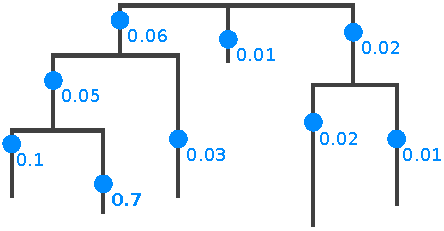
\includegraphics[width=.6\linewidth]{pppp/tree_epa.pdf}
    \caption[Phylogenetic Placement of a Query Sequence]{
        \textbf{Phylogenetic Placement of a Query Sequence.}
        Each branch of the reference tree is tested as a potential insertion position, called a ``placement'' (blue dots).
        Note that placements have a specific position on their branch, due to the branch length optimization process.
        A probability of how likely it is that the sequence belongs to a specific branch is computed
        (numbers next to dots),
        which is called the \emph{likelihood weight ratio} (LWR).
%         based on the maximum likelihood score of the whole tree. %(that is, including the query sequence)
        The bold number (0.7) denotes the most probable placement of the sequence.
    }
    \label{fig:tree_epa}
\end{figure}

This process is repeated for every \ac{QS}.
Note that the placement process is conducted {\em independently} for each \ac{QS}.
% Shorter: This placement process is conducted independently for each sequence.
That is, for each \ac{QS}, the algorithm starts calculating placements from scratch on the original \ac{RT}.
%This enables parallelization,
%and avoids unstable trees, which might result from adding too many sequences of short length to the tree.

In summary, the result of a phylogenetic placement analysis is a mapping of the \acp{QS} in a sample
to positions on the branches of the \ac{RT}.
Each such position, along with the corresponding \ac{LWR}, is called a placement of the \ac{QS}.
% The result of phylogenetic placement is a mapping of each \ac{QS} (e.g., environmental reads)
% to positions on the branches of the \ac{RT}, amended by probabilities in form of their likelihood weight ratios.
% Each \ac{QS} is thus represented by its placement positions, which are also called its placements.
% along with the respective likelihood weight ratios.f
% total: sum up. placement profile. imbalance. explain in later chapter.
% Here, we use these sample profiles to discover: clusters, correlation with meta-data.

\todo{besser unterbringen}
The data is usually stored in so-called \fileformat{jplace} files \cite{Matsen2012}.

% Each such sample represents a geographical location, a body site, a point in time, etc.
In the following, we represent a sample by the placement locations of its metagenomic \acp{QS},
including the respective per-branch \acp{LWR}.
Furthermore, for a specific analysis, we assume the standard use case,
that is, all placements were computed on the same fixed \acf{RT} and \acl{RA}.


This mapping can be seen as an identification and classification of the \acp{QS} in terms of the \ac{RT},
similar to a taxonomic assignment.
However, phylogenetic placement also allows for more elaborate downstream analyses.
Firstly, the reference tree usually offers a higher resolution than simple per-taxon abundance counts,
and the amount of mapped \acp{QS} per branch can be directly visualized on the \ac{RT} \citep{Mahe2017}.
Secondly, established methods such as Edge PCA and Squash Clustering \citep{Matsen2011a}
allow for identifying subtle differences between distinct samples,
thus enabling comparative studies directly based on phylogenetic placement.
Lastly, we recently proposed novel methods for visualizing and clustering phylogenetic placement data \citep{Czech2018a},
which, for example, can reveal correlations of per-sample meta-data features with sequence abundances.


Furthermore, phylogenetic placement is used in a variety of derived tools,
such as \toolname{(m)PTP} (species delimitation; \cite{Zhang2013,Kapli2017}),
\toolname{SEPP} (boosting; \cite{Mirarab2012}),
\toolname{PhyloSift} (metagenome analysis; \cite{Darling2014}),
\toolname{Sativa} (identification and correction of taxonomically mislabeled sequences; \cite{Kozlov2016})
and \toolname{TIPP} (taxonomic identification and phylogenetic profiling; \cite{Nguyen2014}).

A phylogenetic placement can be carried out {\em if} the \acp{QS} can be aligned to the reference alignment.
Often, barcoding regions such as 16S or 18S are used,
but there also exist studies that use different, or even a set of, maker genes \citep{Sunagawa2013a}.
Furthermore, other types of sequences such as $_{\text{mi}}$tags %\textsubscript{mi}tags
\citep{Logares2014} can be used.

% ======================================================================================================================
%     Placement Pipeline
% ======================================================================================================================

\subsection{Placement Pipeline}
\label{ch:Foundations:sec:PhylogeneticPlacement:sub:PlacementPipeline}


alignting against given ref aln, papara, hmmer

ML method, rappas (aln free)


% ######################################################################################################################
%         Phylogenetic Placement Processing
% ######################################################################################################################

\section{Phylogenetic Placement Processing}
\label{ch:Foundations:sec:PhylogeneticPlacementProcessing}

% thus, wehn dealing with many samples, an imporatn question is how to make them comparable when differing numbres o sequences
% the problem arises because different samples zies. can span many order sof magnitude.
When placing multiple samples, for instance, from different locations,
typically, the same \ac{RT} is used, in order to allow for comparisons of the phylogenetic composition of these samples.
In this context, it is important to consider how to properly normalize the samples.
Normalization is required as the sample size (often also called library size),
that is, the number of sequences per sample, can vary by several orders of magnitude,
due to efficiency variations in the sequencing process or biases introduced by the amplification process.
Selecting an appropriate normalization strategy constitutes a common problem in many metagenomic studies.
The appropriateness depends on data characteristics \cite{Weiss2017}, but also on the biological question asked.
For example, estimating indices such as the species richness are often implemented
via rarefaction and rarefaction curves \cite{Gotelli2001},
which however ignores a potentially large amount of the available valid data \cite{McMurdie2014}.
Furthermore, the specific type of input sequence data has to be taken into account for normalization:
Biases induced by the amplification process can potentially be avoided if, instead of amplicons,
data based on shotgun sequencing are used, such as \textsubscript{mi}tags \cite{Logares2014}.
Moreover, the sequences can be clustered prior to phylogenetic placement analysis,
for instance, by constructing operational taxonomic units (OTUs) \cite{Edgar2010,Mahe2014,Mahe2015,Rognes2016}.
Analyses using OTUs focus on species diversity instead of simple abundances.
OTU clustering substantially reduces the number of sequences,
and hence greatly decreases the computational cost for placement analyses.
Lastly, one may completely ignore the abundances (which are called ``multiplicities'' of placements) of the placed
sequences, reads, or OTUs, and only be interested in their presence/absence when comparing samples.

Which of the above analysis strategies is deployed,
depends on the specific design of the study and the research question at hand.
The common challenge is that the number of sequences per sample differs, which affects most post-analysis methods.
Before introducing our methods,
we therefore explain how the necessary normalizations of sample sizes can be performed in the following.
We also describe general techniques for interpreting and working with phylogenetic placement data.
%These are not methods of their own, but tools necessary for later.
Some of these techniques have been used before as building blocks
for methods like Edge PCA and Squash Clustering \cite{Matsen2011a,Evans2012}. \todo{see below}
%and we mostly stick to established terminology.

% ======================================================================================================================
%     Edge Masses
% ======================================================================================================================

\subsection{Edge Masses}
\label{ch:Foundations:sec:PhylogeneticPlacementProcessing:sub:EdgeMasses}

Methods that compare samples directly based on their sequences,
such as the UniFrac distance \cite{Lozupone2005,Lozupone2007a},
can benefit from rarefaction \cite{Weiss2017}.
However, in the context of phylogenetic placement, rarefaction is not necessary.
Thus, more valid data can be kept.
% Directly comparing individual anonymous sequences can be too computationally demanding for large contemporary metagenomic datasets.
% hence, the quantitative methods we present here do not consider the \acp{QS} individually.
% as contemporary metagenomic datasets are often too large to allow for this level of granularity,
To this end, it is convenient to think of the reference tree as a graph
(when exploiting graph properties of the tree, we refer to the branches of the tree as edges).
Then, the per-branch \acp{LWR} for a single \ac{QS}
can be interpreted as mass points distributed over the edges of the \ac{RT},
including their respective placement positions on the branches,
cf.~\figref{fig:tree_epa}.
This implies that each \ac{QS} has a total accumulated mass of $1.0$ on the \ac{RT}.
We call this the \emph{mass interpretation} of the placed \acp{QS}, and henceforth use mass and \ac{LWR} interchangeably.
The \emph{mass of an edge} refers to the sum of the \acp{LWR} on that edge for all \acp{QS} of a sample,
as shown in \figref{fig:imbalance:sub:ReferenceTree}.
The total mass of a sample is then the sum over all edge masses,
which is identical to the number of \acp{QS} in the sample.
% \todo{This neglects that not all placements are stored in jplace, so that the mass per QS can be $<1$.
% This fact is not necessary for explaining any of the methods (although it is accounted for in my implementation).
% I think we can thus omit it for simplicity.}

\begin{figure}[!ht]
    \centering
    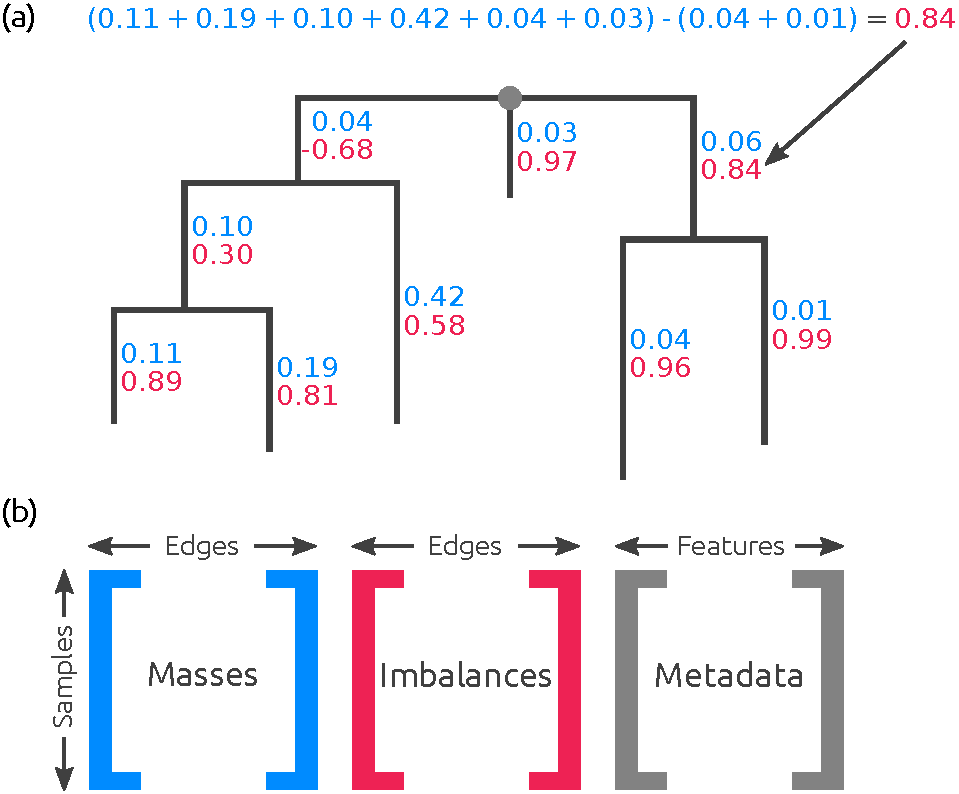
\includegraphics[width=0.8\linewidth]{imbalance.pdf}
    \begin{subfigure}{0pt}
        \phantomcaption
        \label{fig:imbalance:sub:ReferenceTree}
    \end{subfigure}
    \begin{subfigure}{0pt}
        \phantomcaption
        \label{fig:imbalance:sub:Matrices}
    \end{subfigure}
    \caption[Edge Masses and Imbalances]{
        \textbf{Edge Masses and Imbalances.}
        \subref{fig:imbalance:sub:ReferenceTree}
        Reference tree where each edge is annotated with the normalized mass (first value, blue) and
        imbalance (second value, red) of the placements in a sample.
        The imbalance is the sum of masses on the root side of the edge minus the sum of the masses on the non-root side.
        The depicted tree is unrooted, hence, its top-level trifurcation (gray dot) is used as ``root'' node.
        An exemplary calculation of the imbalance is given at the top.
        Because terminal edges only have a root side, their imbalance is not informative.
        \subref{fig:imbalance:sub:Matrices}
        The masses and imbalances for the edges of a sample constitute the rows of the first two matrices.
        The third matrix contains the available meta-data features for each sample.
        These matrices are used to calculate, for instance, the edge principal components or correlation coefficients.
    }
    \label{fig:imbalance}
\end{figure}

The key idea is to use the distribution of placement mass points over the edges of the \ac{RT} to characterize a sample.
This allows for normalizing samples of different size
by scaling the total sample mass to unit mass $1.0$.
In other words, absolute abundances are converted into relative abundances.
This way, rare species, which might have been removed by rarefaction, can be kept,
as they only contribute a negligible mass to the branches into which they have been placed.
This approach is analogous to using proportional values for methods based on OTU count tables,
that is, scaling each sample/column of the table by its sum of OTU counts \cite{Weiss2017}.
% In the following, we will mostly work with normalized samples.
Most of the methods presented here use normalized samples, that is, they use relative abundances.
As relative abundances are compositional data, certain caveats occur \cite{Aitchison1986,Lovell2015},
which we discuss where appropriate.

When working with large numbers of \acp{QS},
the mass interpretation allows to further simplify and reduce the data:
The masses on each edge of the tree can be quantized into $b$ discrete bins,
that is, each edge is divided into $b$ intervals (or bins) of the corresponding branch length.
All mass points on that edge are then accumulated into their respective nearest bin.
% , for example, at their nearest interval midpoint.
% Using midpoints means that masses are only minimally moved.
The parameter $b$ controls the resolution and accuracy of this approximation.
In the extreme case $b:=1$, all masses on an edge are grouped into one single bin.
This \emph{branch binning} process drastically reduces the number of mass points
that need to be stored and analyzed in several methods we present,
while only inducing a negligible decrease in accuracy.
As shown in \tabref{tab:hmp_binning_error}.
branch binning can yield a speedup of up to 75\% for post-analysis run-times.

Furthermore, using masses allows to summarize a set of samples
by annotating the \ac{RT} with their average per-edge mass distribution.
This procedure, also called \emph{squashing} \cite{Matsen2011a}, sums over all sample masses per edge
and then normalizes them once more to obtain unit mass for this resulting average tree.
This normalized tree thereby summarizes the (sub-)set of samples it represents.

% ======================================================================================================================
%     Edge Imbalances
% ======================================================================================================================

\subsection{Edge Imbalances}
\label{ch:Foundations:sec:PhylogeneticPlacementProcessing:sub:EdgeImbalances}

So far, we have only considered the per-edge masses.
Often, however, it is also of interest to ``summarize'' the mass of an entire clade. %, that is, to consider per-clade masses.
For example, sequences of the \ac{RT} that represent species or strains might not provide sufficient phylogenetic signal
for properly resolving the phylogenetic placement of short sequences \cite{Dunthorn2014}.
In these cases, the placement mass of a sequence can be spread across different edges representing the same genus or species,
thus blurring analyses based on per-edge masses.
% e.g., when using regions of the genome that lack the necessary phylogenetic signal for species delimitation.
% In that case, the distinction between masses on two related species branches ...
% it might be more useful to ``summarize'' the mass for the whole genus, that is, to consider per-clade masses.
% These masses then can be interpreted relative to the masses in the rest of the tree.
% The above visualizations show each edge individually, that is, they do not reveal information about whole clades.
Instead, a clade-based summary can yield clearer analysis results.
It can be computed by using the tree structure to appropriately transform the edge masses.
% The \acp{RT} used for phylogenetic placement are generally unrooted.
% They contain however a special node, the top-level trifurcation,
% which serves as a ``hook'' when drawing and storing the tree, and which we can consider as a root for simplicity.
Each edge splits the tree into two parts, of which only one contains the root (or top-level trifurcation) of the tree.
For a given edge, its mass difference is then calculated by summing all masses in the root part of the tree
and subtracting all masses in the other part,
while ignoring the mass of the edge itself \cite{Matsen2011a}.
% For a given edge, the edge mass difference is calculated as the difference between
% the sum of masses on the root side of the edge and all masses on the other side \cite{Matsen2011a}.
This difference is called the \emph{imbalance} of the edge.
It is usually normalized to represent unit total mass,
as the absolute (not normalized) imbalance otherwise propagates the effects of differing sample sizes all across the tree.
% doesn't matter where the root is, entries will change relative to each other accordingly when re-rooting
An example of the imbalance calculation is shown in \figref{fig:imbalance:sub:ReferenceTree}.
The edge imbalance relates the masses on the two sides of an edge to each other.
This implicitly captures the \ac{RT} topology and reveals information about its clades.
Furthermore, this transformation can also reveal differences in the placement mass distribution
of nearby branches of the tree.
This is in contrast to the KR distance, which yields low values for masses that are close to each other on the tree.
% This is for example useful when the tree contains taxa representing species or even strain level,
% which can often not be resolved using phylogenetic placement,
% e.g., when using regions of the genome that lack the necessary phylogenetic signal for species delimitation.
%Note that, %for normalized samples with unit total mass,
%the imbalance of a leaf edge is simply the total mass of the tree minus the mass of the edge.
% It thus contains mostly irrelevant information and can often be left out.
Examples that illustrate the different use cases for edge mass and edge imbalance metrics are shown in the Results section.

The edge masses and edge imbalances per sample can be summarized by two matrices,
which we use for all further downstream edge- and clade-related analyses, respectively.
In these matrices, each row corresponds to a sample, and each column to an edge of the \ac{RT}.
Note that these matrices can either store absolute or relative abundances,
depending on whether the placement mass was normalized.

Furthermore, many studies provide meta-data for their samples,
for instance, the pH value or temperature of the samples' environment.
Such meta-data features can also be summarized in a per-sample matrix, where each column corresponds to one feature.
The three matrices are shown in \figref{fig:imbalance:sub:Matrices}.
Quantitative meta-data features are the most suitable for our purposes,
as they can be used to detect correlations with the placement mass distributions of samples.
For example, Edge principal components analysis (Edge PCA) \cite{Matsen2011a}
is a method that utilizes the imbalance matrix to detect and visualize edges
with a high heterogeneity of mass difference between samples.
Edge PCA further allows to annotate its plots with meta-data variables, for instance, by coloring,
thus establishing a connection between differences in samples and differences in their meta-data \cite{Srinivasan2012}.
In the following, we propose several new techniques to analyze placement data and their associated meta-data.

% ======================================================================================================================
%     Distance between Samples
% ======================================================================================================================

\subsection{Distance between Samples}
\label{ch:Foundations:sec:PhylogeneticPlacementProcessing:sub:Distances}

kr distance. ref to nh distance?!
\cite{Evans2012}

% ======================================================================================================================
%     Existing Analysis Methods
% ======================================================================================================================

\subsection{Existing Analysis Methods}
\label{ch:Foundations:sec:PhylogeneticPlacementProcessing:sub:ExistingMethods}

squash clustering
edge pca
\cite{Matsen2011a,Evans2012}

we use these methods repeatedly to compare our novel methods to.
